\documentclass[aspectratio=169]{beamer}
\usepackage{geometry}
\usepackage{graphicx}
\usepackage{hyperref}
\usepackage{xcolor}
\usepackage{listings}
\usepackage{tikz}
\usepackage{booktabs}

\usetheme{Madrid}
\usecolortheme{seahorse}
\setbeamertemplate{navigation symbols}{}

\definecolor{secureblue}{RGB}{0,102,204}
\definecolor{securegreen}{RGB}{0,153,76}
\definecolor{secureorange}{RGB}{255,153,0}

\title{SecureJob Platform}
\subtitle{A Secure Job Search and Professional Networking Platform}
\author{CSE 345/545 - Foundations of Computer Security}
\date{\today}
\institute{Computer Science and Engineering}

\begin{document}

\begin{frame}
\titlepage
\end{frame}

\begin{frame}{Outline}
\tableofcontents
\end{frame}

\section{Project details}

\begin{frame}{Project Overview}
\begin{columns}
\column{0.5\textwidth}
\textbf{What is SecureJob?}
\begin{itemize}
    \item Comprehensive job search platform
    \item Professional networking features
    \item Security-first design approach
    \item Enterprise-grade protection
\end{itemize}

\column{0.5\textwidth}
\textbf{Key Objectives}
\begin{itemize}
    \item Connect job seekers with recruiters
    \item Protect user data and communications
    \item Implement robust security measures
    \item Ensure privacy compliance
\end{itemize}
\end{columns}
\end{frame}

\begin{frame}{Technology Stack}
\begin{center}
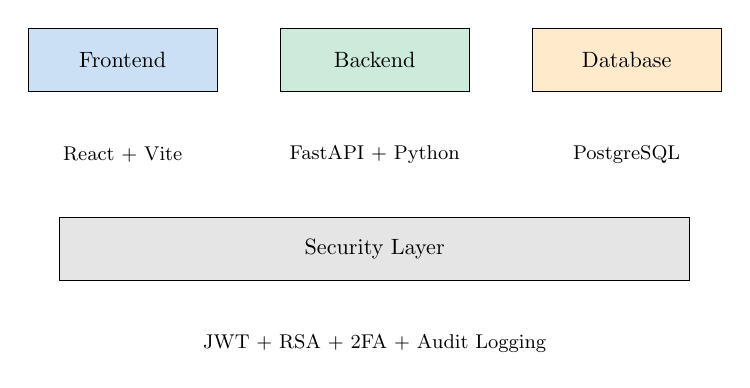
\begin{tikzpicture}[scale=0.8, transform shape]
    \node[draw, fill=secureblue!20, minimum width=3cm, minimum height=1cm] (frontend) at (0,3) {Frontend};
    \node[draw, fill=securegreen!20, minimum width=3cm, minimum height=1cm] (backend) at (4,3) {Backend};
    \node[draw, fill=secureorange!20, minimum width=3cm, minimum height=1cm] (database) at (8,3) {Database};
    
    \node[below of=frontend, node distance=1.5cm] {\small React + Vite};
    \node[below of=backend, node distance=1.5cm] {\small FastAPI + Python};
    \node[below of=database, node distance=1.5cm] {\small PostgreSQL};
    
    \node[draw, fill=gray!20, minimum width=10cm, minimum height=1cm] (security) at (4,0) {Security Layer};
    \node[below of=security, node distance=1.5cm] {\small JWT + RSA + 2FA + Audit Logging};
\end{tikzpicture}
\end{center}
\end{frame}

\begin{frame}{Security Architecture}
\begin{columns}
\column{0.5\textwidth}
\textbf{Defense-in-Depth Approach}
\begin{itemize}
    \item Authentication: JWT-based
    \item Authorization: RBAC
    \item Encryption: End-to-end
    \item Audit: Tamper-evident
    \item Privacy: Granular controls
\end{itemize}

\column{0.5\textwidth}
\textbf{Security Features}
\begin{itemize}
    \item Multi-factor authentication
    \item RSA key pairs for users
    \item Encrypted messaging
    \item Rate limiting
    \item Input validation
    \item SQL injection prevention
\end{itemize}
\end{columns}
\end{frame}

\begin{frame}{Authentication \& Authorization}
\begin{center}
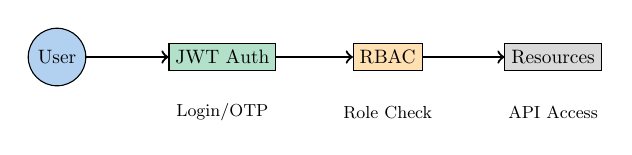
\begin{tikzpicture}[scale=0.7, transform shape]
    \node[draw, circle, fill=secureblue!30] (user) at (0,0) {User};
    \node[draw, rectangle, fill=securegreen!30] (auth) at (3,0) {JWT Auth};
    \node[draw, rectangle, fill=secureorange!30] (rbac) at (6,0) {RBAC};
    \node[draw, rectangle, fill=gray!30] (resource) at (9,0) {Resources};
    
    \draw[->, thick] (user) -- (auth);
    \draw[->, thick] (auth) -- (rbac);
    \draw[->, thick] (rbac) -- (resource);
    
    \node[below of=auth, node distance=1cm] {\small Login/OTP};
    \node[below of=rbac, node distance=1cm] {\small Role Check};
    \node[below of=resource, node distance=1cm] {\small API Access};
\end{tikzpicture}
\end{center}

\vspace{0.5cm}
\textbf{User Roles:}
\begin{itemize}
    \item Job Seekers: Browse jobs, apply, manage profiles
    \item Recruiters: Post jobs, review applications
    \item Administrators: Platform oversight, audit logs
\end{itemize}
\end{frame}

\begin{frame}{Technical Implementation}
\begin{columns}
\column{0.5\textwidth}
\textbf{Backend Architecture}
\begin{itemize}
    \item \textbf{Framework}: FastAPI
    \item \textbf{Language}: Python 3.11
    \item \textbf{Database}: PostgreSQL
    \item \textbf{ORM}: SQLAlchemy
    \item \textbf{Auth}: JWT + OAuth2
\end{itemize}

\column{0.5\textwidth}
\textbf{Frontend Architecture}
\begin{itemize}
    \item \textbf{Framework}: React 18
    \item \textbf{Build System}: Vite
    \item \textbf{Styling}: Tailwind CSS
    \item \textbf{State Management}: Context API
    \item \textbf{Routing}: React Router
\end{itemize}
\end{columns}

\vspace{0.3cm}
\begin{block}{Security Integration}
All components implement security-first design with proper authentication, authorization, and data protection.
\end{block}
\end{frame}

\begin{frame}{Deployment Architecture}
\begin{center}
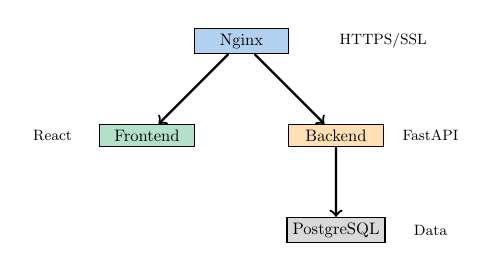
\begin{tikzpicture}[scale=0.6, transform shape]
    \node[draw, rectangle, fill=secureblue!30, minimum width=2cm] (nginx) at (0,0) {Nginx};
    \node[draw, rectangle, fill=securegreen!30, minimum width=2cm] (frontend) at (-2,-2) {Frontend};
    \node[draw, rectangle, fill=secureorange!30, minimum width=2cm] (backend) at (2,-2) {Backend};
    \node[draw, rectangle, fill=gray!30, minimum width=2cm] (database) at (2,-4) {PostgreSQL};
    
    \draw[->, thick] (nginx) -- (frontend);
    \draw[->, thick] (nginx) -- (backend);
    \draw[->, thick] (backend) -- (database);
    
    \node[right of=nginx, node distance=3cm] {\small HTTPS/SSL};
    \node[left of=frontend, node distance=2cm] {\small React};
    \node[right of=backend, node distance=2cm] {\small FastAPI};
    \node[right of=database, node distance=2cm] {\small Data};
\end{tikzpicture}
\end{center}

\vspace{0.3cm}
\textbf{Containerization:}
\begin{itemize}
    \item Docker multi-stage builds
    \item SSL certificate generation
    \item Automated deployment
    \item Environment isolation
\end{itemize}
\end{frame}

\section{Features and functionalities}

\begin{frame}{User Management}
\begin{columns}
\column{0.6\textwidth}
\textbf{Account Features}
\begin{itemize}
    \item Registration with email verification
    \item Multi-factor authentication (TOTP)
    \item Profile management with privacy controls
    \item Account suspension and deletion
    \item Password reset with OTP verification
\end{itemize}

\column{0.4\textwidth}
\textbf{Privacy Controls}
\begin{itemize}
    \item Profile visibility settings
    \item Data sharing preferences
    \item Communication privacy
    \item Activity tracking opt-out
\end{itemize}
\end{columns}

\vspace{0.3cm}
\begin{alertblock}{Security Note}
All user data is encrypted and access is logged with tamper-evident audit trails.
\end{alertblock}
\end{frame}

\begin{frame}{Job Marketplace}
\begin{columns}
\column{0.5\textwidth}
\textbf{Job Search \& Discovery}
\begin{itemize}
    \item Advanced search with filters
    \item Location-based search
    \item Remote job options
    \item Salary range filtering
    \item Skill-based matching
    \item Company profiles
\end{itemize}

\column{0.5\textwidth}
\textbf{Application Management}
\begin{itemize}
    \item Online applications
    \item Resume upload
    \item Application tracking
    \item Status notifications
    \item Interview scheduling
    \item Offer management
\end{itemize}
\end{columns}

\vspace{0.3cm}
\begin{block}{Security Feature}
Resume downloads require OTP verification and are access-logged.
\end{block}
\end{frame}

\begin{frame}{Company Management}
\begin{columns}
\column{0.5\textwidth}
\textbf{Employer Tools}
\begin{itemize}
    \item Company profile creation
    \item Job posting management
    \item Application review
    \item Candidate communication
    \item Recruitment analytics
\end{itemize}

\column{0.5\textwidth}
\textbf{Recruitment Features}
\begin{itemize}
    \item Applicant tracking system
    \item Resume search and filtering
    \item Interview scheduling
    \item Offer management
    \item Bulk communication
\end{itemize}
\end{columns}

\vspace{0.3cm}
\begin{exampleblock}{Access Control}
Company management restricted to authorized recruiters and administrators.
\end{exampleblock}
\end{frame}

\begin{frame}{Professional Networking}
\begin{center}
\textbf{Secure Communication System}
\end{center}

\begin{columns}
\column{0.5\textwidth}
\textbf{Networking Features}
\begin{itemize}
    \item Professional connections
    \item Connection requests
    \item Referral system
    \item Network-based recommendations
\end{itemize}

\column{0.5\textwidth}
\textbf{Secure Messaging}
\begin{itemize}
    \item End-to-end encryption
    \item Digital signatures
    \item Secure file sharing
    \item Conversation management
\end{itemize}
\end{columns}

\vspace{0.3cm}
\begin{exampleblock}{Encryption Details}
Each user has RSA key pairs for message encryption and digital signatures.
\end{exampleblock}
\end{frame}

\begin{frame}{Resume Management}
\begin{columns}
\column{0.5\textwidth}
\textbf{Document Security}
\begin{itemize}
    \item Encrypted resume storage
    \item Secure download with OTP verification
    \item File integrity verification
    \item Access logging and audit trails
\end{itemize}

\column{0.5\textwidth}
\textbf{Resume Features}
\begin{itemize}
    \item Multiple resume formats support
    \item Resume parsing and analysis
    \item Skills extraction and matching
    \item Resume visibility controls
\end{itemize}
\end{columns}

\vspace{0.3cm}
\begin{alertblock}{Security Implementation}
All resume operations require proper authentication and are logged for security monitoring.
\end{alertblock}
\end{frame}

\begin{frame}{Data Protection}
\begin{columns}
\column{0.5\textwidth}
\textbf{Encryption}
\begin{itemize}
    \item RSA key pairs per user
    \item Encrypted data storage
    \item Secure key management
    \item End-to-end messaging
\end{itemize}

\column{0.5\textwidth}
\textbf{Access Control}
\begin{itemize}
    \item Role-based permissions
    \item API rate limiting
    \item IP-based restrictions
    \item Session management
\end{itemize}
\end{columns}

\vspace{0.3cm}
\begin{block}{Compliance}
\begin{itemize}
    \item GDPR compliance features
    \item Data retention policies
    \item User consent management
    \item Audit trail maintenance
\end{itemize}
\end{block}
\end{frame}

\begin{frame}{Audit \& Monitoring}
\begin{center}
\textbf{Tamper-Evident Audit System}
\end{center}

\begin{columns}
\column{0.6\textwidth}
\textbf{Audit Features}
\begin{itemize}
    \item Comprehensive action logging
    \item Hash chain verification
    \item Tamper detection
    \item Admin oversight
    \item Compliance reporting
\end{itemize}

\column{0.4\textwidth}
\textbf{Monitored Events}
\begin{itemize}
    \item User registration
    \item Login attempts
    \item Profile changes
    \item Job applications
    \item Admin actions
\end{itemize}
\end{columns}

\vspace{0.3cm}
\begin{exampleblock}{Security Benefit}
All audit logs are cryptographically chained to prevent tampering.
\end{exampleblock}
\end{frame}

\begin{frame}{Privacy Controls}
\begin{columns}
\column{0.5\textwidth}
\textbf{Privacy Settings}
\begin{itemize}
    \item Profile visibility controls
    \item Data sharing preferences
    \item Communication privacy
    \item Activity tracking opt-out
    \item Search visibility
\end{itemize}

\column{0.5\textwidth}
\textbf{Data Rights}
\begin{itemize}
    \item Right to deletion
    \item Data export functionality
    \item Profile view controls
    \item Consent management
    \item Access logs
\end{itemize}
\end{columns}

\vspace{0.3cm}
\begin{alertblock}{Privacy by Design}
All features implement privacy-first principles with user consent at the core.
\end{alertblock}
\end{frame}

\section{Allegations and Rebuttals for Group 25}

\begin{frame}[fragile]{Security Allegations Summary}
\renewcommand{\arraystretch}{1.2}
\scriptsize
\begin{tabular}{|p{2.8cm}|p{4cm}|p{1.5cm}|p{5.5cm}|}
\hline
\textbf{Reporter} & \textbf{Allegation} & \textbf{Status} & \textbf{Rebuttal} \\
\hline
Mohit Bhariya & Connection requests not working & Partially Valid & Creation works, accept/reject has frontend UI bug \\
\hline
Divjot Flora & IDOR via job modification & Invalid & Job postings are public by design \\
\hline
Divjot Flora & Negative salary values & Valid & Numeric validation needed \\
\hline
Ritviek Padda & Public API docs & Invalid & Informational, not security flaw \\
\hline
Ritviek Padda & User data leakage & Invalid & Public profiles with privacy controls \\
\hline
Ashil Krishna PS & Input validation failure & Partially Invalid & No data corruption, some UI issues \\
\hline
Ashil Krishna PS & Missing E2EE & Valid (Partial) & TLS protects transport, but E2EE gap exists \\
\hline
Angadjeet Singh & User enumeration & Invalid & Public profiles by design, RSA keys meant to be public \\
\hline
Alabhya Jha & JWT in localStorage & Valid & Security risk if XSS occurs \\
\hline
Kartik Kumar Singh & Slowloris DoS & Valid & Confirmed DoS vulnerability \\
\hline
\end{tabular}
\end{frame}

\begin{frame}[fragile]{Additional Allegations}
\renewcommand{\arraystretch}{1.2}
\scriptsize
\begin{tabular}{|p{2.8cm}|p{4cm}|p{1.5cm}|p{5.5cm}|}
\hline
\textbf{Reporter} & \textbf{Allegation} & \textbf{Status} & \textbf{Rebuttal} \\
\hline
Ayush Kumar & Connection request IDs & Valid & Accept/decline flow needs integration fixes \\
\hline
Priyanshu Gupta & Password reset UX & Partially Valid & Logic works, UI response broken \\
\hline
Mohit Bhariya & Recruiter features & Invalid & Requirements substantially satisfied \\
\hline
Ashil Krishna PS & Company creation & Invalid & Works in testing, insufficient evidence \\
\hline
Ashil Krishna PS & Supabase dependency & Invalid & No external auth dependency \\
\hline
Ashil Krishna PS & Clickjacking & Invalid & Insufficient PoC provided \\
\hline
Nitin Rayal & Company creation & Invalid & Works, not reliably reproduced \\
\hline
Nitin Rayal & JWT localStorage & Invalid & Insufficient exploit demonstration \\
\hline
\hline
\end{tabular}

\vspace{0.3cm}
\begin{block}{Summary}
\begin{itemize}
    \item \textbf{Valid Issues}: 6 (connection UI, salary validation, E2EE gap, JWT storage, DoS, password reset UX)
    \item \textbf{Invalid Issues}: 13 (misunderstood features, insufficient evidence, by-design behavior)
    \item \textbf{Partially Valid}: 3 (UI issues, input sanitization)
\end{itemize}
\end{block}
\end{frame}

\section{Conclusion}



\end{document}
